\cotefile{156-5}
\scanpage{18}\mspage{17}
\deleted{\unsure{14|4}} \uline{15 juin}

On peut remplacer $\unsure{\mathcal F|\mathscr F}$ par divers\deleted{\unsure{es}} \inserted{\unsure{p. ex. que : un|pr. ex. un}} sous-ensembles ordonnés, stables \uline{par} \deleted{$\unsure{\in}$} \deleted{et} \deleted{par \unsure{Sup}}
sous-figures \deleted{fermées}\inserted{(i.e. fermés dans $\mathcal F$)} et par $\unsure{\mathrm{Sup}|\inf}$.

Exemples : Si $\unsure{\mathcal L|\mathscr L}$ est un \unsure{esp.} \unsure{top.} \inserted{(\unsure{structuré|str. top.})}, \deleted{\unsure{de}}
on peut soumettre les $A\in F$ \deleted{\unsure{figur}} ($F$ \unsure{figure|figures})
à des conditions de nature topologiques, comme d'être fermés, ou \deleted{\illegible{1}} compacts, ou fermés et connexes. Toute condition
portant sur la nature des strates $A\in F$ (en tant que \unsure{partie} de $L$, et non en tant que multistrate\ldots), ou $=$ sur la nature des
multistrates $F_A$ $(A\in F)$, définit une sous ens. ordonné de $\mathcal F$ ayant les propriétés de stabilité voulues. Signalons ici
des propriétés \unsure{portant} sur \unsure{la|le} $A^\circ=A\setminus\delta A$ (la définition de $A^\circ$ dépend de la multistrate $F_A$), comme celle d'être \deleted{non vide} \deleted{\unsure{connexé|connexe}},
\deleted{\unsure{ou}} \deleted{\unsure{ou}} connexe, ou plus gén. $i$-connexe $\unsure{-1|0}\leq i\leq+\infty$, \deleted{\unsure{$(-1)$-connexe signifiant non vide}} \inserted{et idem pour les $A$ eux-mêmes}. Ou on peut demander aux $|\delta A|$
d'être des sphères topologiques etc.
% slanted
\margin{\uline{NB} \deleted{Mais \unsure{l'énoncé|l'axiome} de \unsure{fi.|pr.} \unsure{supposé} d'\unsure{emblée}, -- peut-être \unsure{a-t-on|stat.}, ou \unsure{même} \unsure{ceci}, \unsure{ne|de} \unsure{saurait}-il \unsure{même} \unsure{convenir|voir} \unsure{en} \unsure{spécifiant} \unsure{cette} \unsure{notion} \unsure{avec|sur} des \unsure{fig.} \unsure{ou|un} $\unsure{F}$ \unsure{seulement} \uline{\unsure{préadmissibles}}.} Aussi, la condition de \uline{densité} $A=\overline{A^\circ}$ i.e. $A\subset B\Longrightarrow A^\circ\subset\overline{B^\circ}$.}

Si $\mathcal L$ \unsure{est} \inserted{un espace} modéré, on se borne aux $\unsure{\Phi|\mathit{\Phi}}\subset\unsure{\mathcal P|\mathfrak P}(\mathcal L)$ pour lesquels $A\in\Phi\Longrightarrow A$ partie fermée \uline{\unsure{par ordre|pour ordre|par ordinaire}} de $L$

On peut envisager aussi des conditions de nature plus globale sur $\Phi$, au cas où
\scanpage{19}\mspage{18}
$L$ est muni d'une topologie, comme celle d'être \uline{localement} fini. Le sous-ens.
ordonné ${\unsure{\mathcal F|\mathscr F}}'$ \deleted{\unsure{de}} $\mathcal F$ est alors stable par sup \unsure{finis|fini}, mais pas \deleted{\unsure{par}} \unsure{généralt} par \unsure{sup.|Inf.}
quelc. \uline{Figure finie} $F$ : \deleted{\unsure{finie}} $F$ fini au sens ordinaire, i.e. un \unsure{nb|ens} fini de strates. Figure de type fini : contenue
dans une réunion finie de ss-figures $F_A$.

\deleted{Si les strates d'une} Une figure est \deleted{\unsure{de t.}} finie \deleted{\unsure{si}} si et \unsure{seult|seulement} si elle est de t. f. et ses strates sont finies.

Autre cas : supposons $L$ muni d'une structure d'ordre -- \unsure{il|et} \unsure{--|a} \unsure{dans|donné} une réalisation topologique, par des ``\uline{cellules}'' \inserted{(fermées) $X_x$ $(x\in L)$} dans un espace
top. $X$ triangulé convenable. Alors à tout $A\deleted{\unsure{\in}}\unsure{\subset|\in}L$ correspond \deleted{\unsure{le}} $X_A=\bigcup_{x\in A}X_x$.
% slanted
\margin{les $X_x$ forment une \uline{famille} admissible de parties de $X$, indexée par l'ens ordonné $L$}
On se bornera alors \unsure{alors} aux parties \uline{fermées} $A$ de $L$, de façon que
\[ A\longmapsto X_A \]
soit une application \unsure{bijective|bijection} de l'ens des parties envisagées de $L$ (les p. \uline{fermées})
\deleted{\unsure{dans l'}}\inserted{\unsure{sur un|avec un}} ens des parties \inserted{fermées} de $X$ \deleted{\unsure{stables}} \deleted{par la relation} \inserted{stables par la} relation d'équivalence \unsure{induite} par \deleted{\unsure{les}} $(X_x^\circ)_{x\in L}$ (en fait, toutes les parties
\scanpage{20}\mspage{19}
de ce type si $L$ est fini). Donc on se bornera donc aux $\unsure{\Phi|\mathit{\Phi}}\in\unsure{\mathcal F|\mathscr F}$ telles que les $A\in\Phi$ soient fermés de $L$, i.e. telle que
\[ \Phi\subset\unsure{\mathcal P|\mathfrak P}_{\text{fermés}}(L) \]
Les \unsure{élément|éléments} de $\mathcal F'$ ainsi \unsure{obtenu|obtenus} peuvent s'interpréter en termes de $X$, comme des familles admissibles \inserted{(\unsure{mais oui|maxim.})} de familles de
parties \inserted{fermées} de $X$, \inserted{chacune} \uline{stables} par la relation d'équiv. des \deleted{cellules} \inserted{strates} ouvertes $X_{\unsure{\circ|a|\bullet|\cdot}}^\circ$, i.e. chacune réunion de strates fermées de $X$.
Dans une terminologie qui sera développée, elles \deleted{sont}\inserted{admettent} donc toutes le recouvrement donné de $X$ comme une ``subdivision''\unsure{,|;} (ou \unsure{plus tôt|plutôt}, \inserted{celui} induit sur leur support dans $X$)

\figure{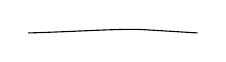
\begin{tikzpicture}\draw (0,0) .. controls (0.7,0.02) and (1.2,0.06) .. (1.5,0.04) -- (2.15,0);\end{tikzpicture}}

Soient $\deleted{\unsure{\Phi}}F$ et $G$ deux figures ensemblistes de $L$. On \unsure{veut|sait|va} définir quand $F$ est un \uline{raffinement}, et quand c'est une \uline{subdivision} de $G$.

\uline{Proposition} Conditions équivalentes

% slanted
\margin{Cela implique $|\deleted{\unsure{A}}F|\subset|G|$}
a) $[$ $\forall\unsure{a|\cdot}\;A\in F$, désignant par $G\deleted{{}_A}{}^A$ l'ens des $B\in G$ tels que $A\subset B$, $G\deleted{{}_A}{}^A$ a un plus petit
élément $\varphi(A)$. (On trouve donc une application $\varphi:\deleted{\unsure{A}}F\longrightarrow G$, qui est bien sur croissante.) $]$ De plus
\scanpage{21}\mspage{20}
pour tout $A\in F$, $B\in G$, $A\cap F$ est \deleted{réunion de}\inserted{une} partie $F$-fermée de $|F|$, i.e. réunion de strates de $F$.
% slanted
\margin{\uline{NB} Le ``de plus'' implique déjà la première condition, si on \unsure{ajoute|a joint} que $|\deleted{\unsure{A}}F|\subset|\deleted{\unsure{B}}G|$, et cela équivaut à $|F|\unsure{-|\longrightarrow}|G|$ \uline{continue} (ou croissante).}\margin{Cf la condition $\mathrm{b}'$) \unsure{équivalente} à la page suivante}

b) Pour tout $A\in F$, $\exists\,B\in G$ telle que $A^\circ\subset B^\circ$ (\unsure{strate} \unsure{évidemt} unique, \inserted{\unsure{noté|notée|soit} $\varphi(A)$}), l'application $\varphi:\deleted{\unsure{F}}F\unsure{-|\longrightarrow}G$ ainsi obtenue est croissante (
\deleted{$A'\subset A$, et} \deleted{$A'^\circ\in\unsure{+|F}$} \deleted{$A'\subset A$} $A,\deleted{\unsure{B}}A'\in F$, $\deleted{\unsure{A'}}B,B'\in G$, \deleted{$A\unsure{=|\subset} A'$, $A^\circ\subset B^\circ$, $\unsure{B\subset B'}$} \unsure{avec} $A^\circ\subset B^\circ$, $A'^\circ\subset B'^\circ$, $A'\subset A$, $\Longrightarrow B'\subset B$.

a) $\Longrightarrow$ b) Supposons a) prouvons b). Soit $A\in F$, \deleted{\unsure{par}} a) $\exists\ B\inserted{{}=\varphi(A)}\in G$ \deleted{tel} qui soit plus petit \unsure{ds|des|dans} $G^A$. Prouvons $\deleted{\unsure{B}}A^\circ\subset B^\circ$. Soit
$x\in A^\circ$, il faut prouver que $B'\in G$, $B'\deleted{\unsure{\in}}\unsure{\subset|\not\subset} B$ et $x\in B'\Longrightarrow B'=B$. \deleted{Soit} Considérons $B'\cap A$, c'est une partie de $A$ réunion \unsure{de'|de} strates de $F$,
donc $\exists\ A'\in\deleted{\unsure{\Phi}}F$, telle que $x\in A'\subset B'\cap A$. Comme $x\in A^\circ$ et $A'\in\deleted{\unsure{\Phi}}F_A$, on a $A'=A$ et comme $A'=A\subset B'\cap A$, on a $A\subset B'$. D'après le caractère minimal de
$B^{\unsure{s|'}}$, on a donc $B'=B$ \unsure{qed.} / D'autre part, on a déjà noté que l'application $\varphi$ est croissante. \deleted{\unsure{Donc}}Cela établit b).

b) $\Longrightarrow$ a). Supposons b, prouvons a). Soit $A\in F$, soit $B\in G$ telle que $A^\circ\subset B^\circ$, prouvons que $B$ est plus petit \inserted{élémt} dans $G^A$.
% slanted
\margin{\uline{Lemme} Moyennant b) on a \unsure{(b)} : Si $A\in F$, $B\in G$, $A^\circ\subset B$ alors $A\subset B$}
Prouvons déjà que $B\in G^A$, i.e. $A\subset B$ \deleted{\unsure{soit|Soit} $B'\in G$ tel que $A\subset B'$}
\deleted{Soit} On a $A=\deleted{\bigcup_{\unsure{A'}}\unsure{A^\circ}\unsure{\in|\subset}\unsure{\sim}}\bigcup_{\substack{A'\in F\\ A'\unsure{\subset|\in} A}} A'^\circ$, \deleted{Comme $A^\circ\subset B^\circ\subset B$,} il suffit de prouver que \unsure{les} $A'^\circ$ sont $\subset B$
\scanpage{22}\mspage{21}
Or si $B'\in G$ est tel que $A'^\circ\subset B'^\circ$, on a \deleted{$\unsure{A}\subset B'$} (hyp. de b) $B'\subset \deleted{\unsure{A}}B$, donc $A'^\circ\subset B$, OK.

Prouvons que $B$ est le plus petit él. de $G^A$. Soit $B'\in G^A$ i.e. $B'\in G$, $A\subset B'$, prouvons $B\subset B'$ ou encore $B^\circ\deleted{\unsure{\subset}}\cap B'\ne\varnothing$ \deleted{\unsure{Comme}}. Comme
$A^\circ\subset B^\circ$ et $A^\circ\subset A\subset B'$, on a $\underset{\substack{\mathrel{\ooalign{\hfil$\scriptstyle\shortparallel$\hfil\cr\hfil$\scriptstyle-$\hfil\cr}}\\ \varnothing}}{A^\circ}\subset B^\circ\cap B'$, OK.

Prouvons enfin que $A\in F$, $B\in G$ implique que $A\cap B$ est $F$ fermé \unsure{dans|ds|de} $|F|$. Par b) on voit que $\underset{\substack{\shortparallel\\ \bigcup_{A\in F}A^\circ}}{|F|}\subset|G|$, et que
la relation d'équiv. $\unsure{\mathcal R|R}_F$ sur $|F|$ est plus fine que celle induite par $\mathcal R_G$ sur $|G|$. Cela implique que $A\cap B$ est saturée pour la relation d'équiv. $\deleted{\unsure{F}}\mathcal R_F$ (puisque $B$ l'est pour $\mathcal R_G$). Donc
\[ A\cap B=\bigcup_{\substack{C\in F\\ \text{t.q. } C^\circ\subset A\cap B}} C^\circ . \]
Je dis que \inserted{dans} cette réunion, \deleted{\unsure{est}} on peut remplacer $C^\circ$ par $C$ i.e.
\[ C\in F,\quad C^\circ\subset A\cap B\quad\Longrightarrow\quad C\subset A\cap B. \]
Comme $C^\circ\subset A$, on a $C\deleted{\unsure{{}^\circ}}\subset A$. Reste : prouver $C\subset B$. On va donner un complément \unsure{immédiat|inédit} à l'énoncé de la prop.
% slanted
\margin{Ou encore : ($\mathrm{b}''$) \unsure{Ou|On a|On} : $|F|\subset|G|$, la relation de préordre sur $|F|$ définie par $F$ est plus fine que celle induite par la relation \unsure{d'ordre|de préordre} de $|G|$.}

\uline{Corollaire} La condition b) équivaut à
$\mathrm{b}'$) $\forall\ A\in F,\ \exists\ B\in G$ tel que $A^\circ\subset B^\circ$, et d'autre part $A\in F$, $B\in G$, $A^\circ\subset B$ implique $A\subset B$.
\scanpage{23}\mspage{22}
Il nous fallait plutôt $\mathrm b\Rightarrow\mathrm b'$ pour achever la dém. de la prop., \deleted{\unsure{Voici} \unsure{donc} \unsure{le} déjà \unsure{fait}} \inserted{et en fait on l'a déjà} \deleted{donc \unsure{à|:} voir \unsure{(pour}} \deleted{(pour $\mathrm b\Rightarrow\mathrm b'$) que}
\deleted{moyennant b), \unsure{on}}
\[ \deleted{A\in F,\quad B\in G,\quad A^\circ\subset B\quad\Longrightarrow\quad A\subset B} \]
\deleted{\unsure{On}} \unsure{prouvé|prouvé'} \deleted{\unsure{cel|cela}}\unsure{en} démontrant $\mathrm b)\Rightarrow\mathrm a)$ (Cf lemme marginal p. 20) Reste : prouver $\mathrm b'\Rightarrow\mathrm b$ donc moyennant $\mathrm{b}'$, le fait que $\varphi$ est croissant
\[ A,A'\in F,\quad B,B'\in G,\quad A^\circ\subset B^\circ,\quad A'^\circ\unsure{\subset|\subset'}B'^\circ,\quad \deleted{\Longrightarrow}\inserted{A'\subset A\deleted{{}^{\unsure{\circ|'|*}}}}\quad\Longrightarrow\quad B'\subset B\deleted{{}^{\unsure{\circ|'|*}}} \]
Mais \deleted{\unsure{Comme}} \inserted{par $\mathrm{b}'$) on a} \deleted{$\unsure{A^\circ\subset A^\circ|A^\circ\subset B^\circ}$ donc} \deleted{$A\subset B$, $A'\subset B'$} \deleted{$A'^\circ\subset B'^\circ$, donc par} $A\deleted{{}^{\unsure{\circ}}}\subset B\deleted{{}^{\unsure{\circ}}}$ \deleted{$\mathrm{b}'$) $A'^\circ\subset B'$, \unsure{donc} on a $A'^\circ\subset A'\subset A\subset B$ donc $A'^\circ\subset$} \deleted{$A^\circ\subset B\cap B'$, donc} donc $A'^\circ\subset B'^\circ$ \deleted{$\unsure{\subset B^\circ}\ \unsure{A\subset A'}$}
$A'^\circ\subset A\subset B$, donc $A'^\circ\subset B'^\circ\cap B$, donc $B'^\circ\cap B\ne\varnothing$, donc $B'\deleted{{}^{\unsure{\circ|'|*}}}\unsure{\in|\subset}B$, qed.

\uline{Définition} On dit, sous ces conditions, que $F$ est un \uline{raffinement} de $G$.
% slanted
\margin{\uline{NB} $F$ raffine $G$ \unsure{ssi} $\forall A\in F$, $F_A$ \unsure{raff.|raffine} $G$ i.e. \unsure{tt|toute} multistrate de $F$ raffine $G$.}

\uline{Ex} Toute sous figure de $G$ est un \unsure{raff.}$^{\unsure{t}}$ de $G$
\unsure{Notation} $F\ll G$. C'est \uline{une relation d'ordre}

\uline{Proposition} Soient $F$ et $G$ deux figures, \deleted{telles que $F$ soit un raffinement de $G$.} Conditions équivalentes
a) \inserted{$F\ll G$,} Il n'existe pas de raffinement de $G$ autre que $F$, parmi ceux dont $F$ soit une sous figure -- i.e. $F$ est \unsure{maximal|minimal} dans l'ens des raffinements de $G$, ordonné \unsure{par|pour} $\leq$ (relation de sous figure)
b) \inserted{$F\ll G$ et} $|F|=|G|$ \deleted{c) \unsure{L'applicat|L'applicat.}}
\scanpage{24}\mspage{23}
b) $\Rightarrow$ a) Si $F'$ est un raffinement de $G$ tel que $F'$ sous figure de $F$, on a $|F|\subset|F'|\subset|G|$, et comme $|F|=|G|$ on
a $|F|=|F'|$, donc $F=F'$, puisque $F$ sous-figure de $F'$,
% slanted
\margin{\uline{Donnons aussi} condition \unsure{équiv.} c) \inserted{$F\ll G$ et} Toute strate de $G$ est réunion de strates de $F$. Et quand \unsure{on ne suppose plus|on ne suppose pas} \unsure{par avance|d'avance} que $F\ll G$, la condition d) \[\left\{\begin{aligned}&1^\circ)\ \text{Toute strate de }G\text{ est réunion de strates de }F\\&2^\circ)\ \forall \deleted{\unsure{B}}A\in F,\quad G^A=\{B\in G\mid B\supset A\}\text{ a un}\\&\text{plus petit élément.}\end{aligned}\right.\]}

a) $\Rightarrow$ b) Supposons que $|F|\ne|G|$, \deleted{soit $x\in|G|\setminus|F|$, considérons la} Il existe donc une figure $\deleted{\unsure{F}}H$ \deleted{qui \unsure{soit}} \inserted{telle} que \deleted{\unsure{vide}, qui soit un raffinement de $G$,}
\[ \left\{\begin{aligned} &|H|\ne\varnothing\\ &\deleted{\unsure{F}}H\ \text{raffine }G\\ &\deleted{\unsure{F}}H\ \text{disjointe de }F \end{aligned}\right. \]
par exemple on prend \unsure{un} $x\in|G|\setminus|F|$, et la figure $\deleted{\unsure{F}}H=\{\{x\}\}$. Or on a

\uline{Corollaire}\enspace Soient $F,H$ deux figures qui raffinent $G$, et telles que $F$ et $H$ \deleted{disjointes} \inserted{compatibles}. Alors $F\unsure{\cup|\vee}H$ raffine $G$.
% slanted
\margin{\figure{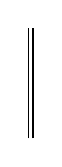
\begin{tikzpicture}\draw (0,0)--(0,1.4) (.06,0)--(.06,1.4);\end{tikzpicture}} à noter \unsure{comme une|car une} propriété formelle intéressante. \unsure{Cas contraire|Au contraire|Par contre} $\pm$ \unsure{génle.} \unsure{Car sinon|Car en somme|(au voisin}, les \unsure{contraires|conditions} \unsure{modérés}) des unions (cas non modéré) si $F$ et $G$ disjointes\ldots}
\inserted{\uline{Plus gén.}, \unsure{ça marche|le même|de même} pour Sup \unsure{quel.|quelc.} (au sens de $\leq$)}
En effet, on utilise le fait que les multistrates de $F\cup H$ sont les multistrates \deleted{qui sont communes à $F$} qui appartiennent à $F$, ou \deleted{\unsure{à}} $H$. Or la propriété de raffinement se vérifie sur les multistrates.

\uline{Définition} On dit alors que $F$ est une \uline{subdivision} de $G$.
\scanpage{25}\mspage{24}
Notation $F\unsure{\preccurlyeq|\preceq}G$. C'est encore une relation d'ordre sur $\unsure{\mathcal F|\mathscr F}$.

\uline{NB} Se donner dans $L$ un couple $F\subset G$, avec $F$ raffinant $G$, revient au $=$ que de se donner
\diagram{\begin{tikzcd}[ampersand replacement=\&,column sep=large,row sep=large]
S\;(=|F|)\arrow[r,hook,"i"]\arrow[d,"p","\text{surj}"'] \& T\;(=|G|)\arrow[r,-,to path={([xshift=4pt,yshift=2pt]\tikztostart.east) .. controls ([xshift=-1pt,yshift=2pt]\tikztostart.east) and ([xshift=-1pt]\tikztostart.east) .. ([xshift=4pt]\tikztostart.east) -- (\tikztotarget.west) -- ([xshift=-2pt,yshift=2pt]\tikztotarget.west)}]\arrow[d,"q"',"\text{surj}"] \& L \\
I\;(=F)\arrow[r,"\varphi"] \& J\;(=G) \&
\end{tikzcd}}
où $S\subset T$ sont des sous. ens. de $L$, $\varphi:I\unsure{\longrightarrow|-}J$ une application \uline{croissante} d'ensembles ordonnés, et \deleted{$\unsure{p}$}
\[p:S-I,\quad q:T-J\]
des appl. \uline{surjectives} ($\varphi$ pas \unsure{néc.|nec.} surjective)

Alors l'inclusion $i$ est continue pour les top. \unsure{corresp|comp|can.} sur $S,T$ définies par leurs préordres respectifs (images inv. des top. sur $I,J$) L'image inverse d'une partie \inserted{$G$-}modérée de $T$ est une partie $F$-modérée de $S$, cette \unsure{notion} se \unsure{raméne|ramène|ramenant} à la \unsure{notion}
\[J'\longrightarrow\varphi^{-1}(J')\]
au niveau des parties de $J,I$. L'image \deleted{\unsure{inv.}}\unsure{dir.|inv.} d'une partie fermée
